\begin{abstract}
We consider a matched subspace detection problem where a signal vector residing in an unknown low-rank $k$ subspace is to be detected using a subspace estimate obtained from noisy signal-bearing training data with missing entries. The resulting subspace estimate is inaccurate due to limited training data, missing entries, and additive noise. Recent results from random matrix theory (RMT) precisely quantify these subspace estimation errors for the setting where the signal has low coherence. We analytically quantify the ROC performance of the resulting plug-in detector and derive a new detector which explicitly accounts for these subspace estimation errors. The realized increase in performance can be attributed to the new detector only using the $k_\text{eff}\leq k$ ``informative'' signal subspace components. The fraction of observed entries determines $k_\text{eff}$ via a simple relationship that we describe. Detection performance better than random guessing is only achievable when the percent of observed data is above a critical threshold which we explicitly characterize.
\end{abstract}
%
\begin{keywords}
Matched subspace detector, random matrix theory, missing data, ROC analysis
\end{keywords}
%
\section{Introduction}\label{sec:intro}

The matched subspace detector (MSD) is a widely used tool in signal processing and machine learning to detect a signal embedded in a low-rank subspace in the presence of additive noise \cite{scharf1994matched,jin2005cfar,mcwhorter2003matched}. The performance of the MSD has been explored when the low-rank signal subspace is known. Scharf and Friedlander \cite{scharf1994matched} consider the MSD when the signal is placed deterministically at an unknown location in a known subspace while McWhorter and Scharf \cite{mcwhorter2003matched} extend this work to allow the signal to be placed randomly with a known (or assumed) distribution in the known subspace.

There is little work characterizing the performance of the matched subspace detector when the signal subspace is unknown and estimated from data. Recently, we used RMT to quantify the performance of stochastic MSDs in such a setting  \cite{asendorf2011msd}. That work brought into sharp focus the importance of using $k_\text{eff}\leq k$ informative signal subspace components in detector statistics; here $k_{\text{eff}}$ is the effective number of informative components identifiable from limited, noisy data as described in \cite{nadakuditi2008sample}. In this paper, we extend the analysis to the deterministic MSD setting where the training data is noisy \textit{and} has missing entries. The missing entry context is motivated in \cite{balzano2010high} by distributed detection scenarios where it might be prohibitive to collect and transmit only a (randomly chosen) fraction $p$ of the training data entries. Alternately one might think of $1-p \in (0,1)$ as a compression factor as in compressed sensing.

The main contribution of this paper is a precise quantification of the resulting performance of the MSD. We uncover a phase transition phenomenon by showing that there is a critical fraction, $p_\text{crit}$, which is a simple function of the eigen-SNR, the number of training samples, and the number of sensors, below which detection performance deteriorates to random guessing. Compressing the training dataset below this critical fraction is undesirable.

The paper is organized as follows. Section \ref{sec:prob stat} formally states the detection problem. Section \ref{sec:rmt} presents pertinent results from RMT. These results are used in Section \ref{sec:derive} to derive a plug-in and random matrix theory MSD and in Section \ref{sec:roc} to derive theoretical ROC curves for each detector. Section \ref{sec:results} validates our analytical predictions, highlights the importance of selecting $k_\text{eff}$ over $k$ subspace components, and demonstrates the effect of missing data. Section \ref{sec:conclusion} presents concluding remarks.

\section{Problem Statement}\label{sec:prob stat}

We consider the detection problem where our observation vector $y \in \mathbb{C}^{n \times 1}$ is modeled as follows:
\begin{equation}\label{eq:problem}
y=\left\{
\begin{aligned}
&z
&& y\in H_0\\
&U\Sigma x+z
&& y\in H_1\\
\end{aligned}\right.
\end{equation}
where $z\sim\mathcal{CN}(0,I_n)$, $U$ is an unknown $n\times k$ (real or complex) matrix with orthonormal columns, $\Sigma=\diag(\sigma_1,\dots,\sigma_k)$ is assumed known with $\sigma_1>\sigma_2>\dots>\sigma_k>0$, and $x\in\mathbb{C}^{k\times 1}$ is an unknown deterministic vector. In the oracle setting, the subspace dimension, $k$, is known with $k\ll n$.

To estimate our unknown subspace, $U$, we are given independent signal-bearing training data $\{y_1,\dots,y_m\}$, such that
\begin{equation}\label{eq:training_data}
y_i = Ux_i + z_i
\end{equation}
where $x_i\overset{\text{i.i.d.}}{\sim}\mathcal{CN}(0,\Sigma^2)$, $z_i\overset{\text{i.i.d.}}{\sim}\mathcal{CN}(0,I_n)$, and $\Sigma$ and $U$ are as defined above; $z_i$ and $x_i$ are independent. We observe only a fraction $p \in (0,1)$ of the entries of the $n \times m$ matrix $Y = \begin{bmatrix} y_1 & \ldots & y_{m} \end{bmatrix}$; $p$ is independent of $n$ and $m$ and we choose which entries are observed at random with i.i.d. probability $p$; the unobserved/missing entries are set to zero.

The resulting matrix is denoted $\widetilde{Y}$. We form our estimate of the signal subspace, $\widehat{U}$, by taking the first $k$ left singular vectors of the SVD of $\widetilde{Y}$. After forming our subspace estimate, $\widehat{U}$,  and given a new (independent) observation $y$ from (\ref{eq:problem}), we generate a $k \times 1$ test vector $w=\widehat{U}^Hy$. Our objective is to formulate a detector, $g(w)\to\{H_0,H_1\}$, which maximizes the probability of detection subject to a specified false alarm rate  $\alpha$.

\section{Pertinent Results from RMT}\label{sec:rmt}

By modifying an argument in  \cite{benaych2011singular}, we obtain the following result.
\begin{Th}\label{th:angles}
Assume that $x_i \sim \mathcal{CN}(0,\Sigma^2)$ as in (\ref{eq:training_data}) and that $U$ in (\ref{eq:training_data}) obeys a low coherence condition. Then as $n,m \longrightarrow \infty$ with $n/m \to c$ we have that for $i,j = 1, \ldots, k$:
\begin{equation*}
\begin{aligned}
&|\langle u_i,\widehat{u}_i\rangle|^2\convas
\begin{cases}
1-\dfrac{c\left(1+p\sigma_i^2\right)}{p\sigma_i^2\left(p\sigma_i^2 + c\right)} & \text{ if } \sigma_{i}>\dfrac{c^{1/4}}{\sqrt{p}}\\
0 & \textrm{otherwise}\\
\end{cases}\\
&|\langle u_i,\widehat{u}_j\rangle|^2\convas 0 \qquad \textrm{ for } i \neq j.\\
\end{aligned}.
\end{equation*}
where $\widehat{u}_i$ are the left singular vectors of $\widetilde{Y}$.
\end{Th}

The low coherence condition appears in, for example, \cite{balzano2010high} with the idea being that the matrix $U \begin{bmatrix} x_{1} & \ldots & x_{m} \end{bmatrix}$ has entries of about the same magnitude. With the Gaussianity assumption for $x$, all we need is $U$ to have low coherence. Recall that the coherence of a matrix with orthonormal columns is $\max_{i,j}|U_{i,j}|$. When a matrix is  spiky, random sampling of its entries may result in a loss of information; matrices with low coherence behave better under random sampling and it is this setting that we focus on in this paper.

The key insight from Theorem \ref{th:angles} is that only the singular vectors corresponding to signal singular values above the phase transition $\frac{c^{1/4}}{\sqrt{p}}$ are \textit{informative}. The fraction of missing entries $p$ regulates this phase transition point as $O(1/\sqrt{p})$. When a signal singular value drops below this critical threshold, the corresponding singular vector estimate is essentially noise-like  (i.e. $|\langle u_i,\widehat{u}_i\rangle|^2=o_{p}(1)$) and thus \textit{uninformative}. The term $|\langle u_i,\widehat{u}_i\rangle|^2$ quantifies mismatch between the estimated and underlying singular vectors;  when $p < p_{\text{crit.}} :=\sqrt{c}/\max_{i}(\sigma_{i}^{2})$ then \textit{all} singular vectors are uninformative. Intuitively we expect a degradation in the performance of detectors  that utilize subspace components for which $|\langle u_i,\widehat{u}_i\rangle|^2=o_{p}(1)$.  We refer to the estimate in Theorem \ref{th:angles} as $|\langle u_i,\widehat{u}_i\rangle|^2_{\text{rmt}}$.

\section{Family of Matched Subspace Detectors}\label{sec:derive}

The Neyman-Pearson solution to the detection problem posed is a likelihood ratio test (LRT)
\begin{equation*}
\Lambda(w) \detgtrless \eta
\end{equation*}
where $\Lambda(w) = \frac{f(w|H_1)}{f(w|H_0)}$ and $\eta$ satisfies $P(\Lambda(w)>\eta|H_0)=\alpha$. The LRT relies on the conditional distributions of our test statistic under each hypothesis, which by properties of Gaussian random variables are simply
\begin{equation*}
\begin{aligned}
&w|H_0\sim\mathcal{N}(0,I_{k})\,\,\,\text{and}\,\,\, w|H_1\sim\mathcal{N}(\widehat{U}^HU\Sigma x, I_{k}).\\
\end{aligned}
\end{equation*}
However, as $x$ is unknown, we employ the generalized likelihood ratio test (GLRT) where $\Lambda(w) = \frac{\max_x f(w|H_1)}{f(w|H_0)}$. The GLRT statistic for our processed data $w$ is
\begin{equation*}
\Lambda(w)=\frac{\max_x\mathcal{N}(\widehat{U}^HU\Sigma x,I_{k})}{\mathcal{N}(0,I_{k})}.
\end{equation*}
Employing maximum likelihood estimation on $x$ yields the estimate $\widehat{x}=\left(\Sigma U^H\widehat{U}\widehat{U}^HU\Sigma\right)^{-1}\Sigma U^H\widehat{U}w$. After simplification of the GLRT using $\widehat{x}$ and using the natural logarithm operator as a monotonic operation, the GLRT statistic becomes
\begin{equation}\label{eq:oracle stat}
\Lambda(w) = w^H\left(\widehat{U}^HU\Sigma\left(\Sigma U^H\widehat{U}\widehat{U}^HU\Sigma\right)^{-1}\Sigma U^H\widehat{U}\right)w.
\end{equation}
%and the detector is $\Lambda(w) \detgtrless 2\ln(\eta)$ where $\eta$ satisfies $P(\Lambda(w)>2\ln\left(\eta\right)|H_0)=\alpha$.

\subsection{Plug-in Detector}

In our problem statement, $U$ is unknown, and therefore (\ref{eq:oracle stat}) cannot be computed directly. One may then substitute a ML estimate for $U$ in (\ref{eq:oracle stat}) as in \cite{jin2005cfar} and \cite{mcwhorter2003matched}. The ML estimate (in the large-sample, small matrix setting) for $U$ is the top $k$ left singular vectors $\widehat{U}=[\widehat{u}_1 \dots \widehat{u}_{k}]$ of the training data matrix, $\widetilde{Y}$.

By replacing $U$ with the estimate $\widehat{U}$ we obtain the plug-in detector which employs the test statistic:
\begin{equation*}
\Lambda_{\text{plugin}}(w)= w^H\left(\widehat{U}^H\widehat{U}\Sigma\left(\Sigma\widehat{U}^H\widehat{U}\widehat{U}^H\widehat{U}\Sigma\right)^{-1}\Sigma\widehat{U}^H\widehat{U}\right)w.\\
\end{equation*}
This simplifies to
\begin{equation}\label{eq:plugin stat}
\boxed{\Lambda_{\text{plugin}}(w) = w^Hw=\sum_{i=1}^kw_i^2}
\end{equation}
and our detector becomes
\begin{equation}\label{eq:plugin classifier}
\boxed{\Lambda_{\text{plugin}}(w) \detgtrless 2\ln(\eta_{\text{plugin}})}
\end{equation}
where $\eta_{\text{plugin}}$ satisfies $P(\Lambda_{\text{plugin}}(w)>2\ln\left(\eta_{\text{plugin}}\right)|H_0)=\alpha$.

The plug-in detector assumes that the estimated signal subspace $\widehat{U}$ is equal to the true signal subspace $U$. However, as shown in Section \ref{sec:rmt}, using uninformative components of $w$ is not well motivated.

\subsection{Random Matrix Theory Detector}\label{subsec:optdet}

Consider the term $\widehat{U}^HU$. By Theorem \ref{th:angles} and by noting that the singular vectors are unique up to a phase, we have that in the large matrix limit $\widehat{U}^HU \approx SA$ where $S=\diag(s_1,\dots,s_{k})$ with $s_i=\exp(j \psi_i)$ where for some $\psi_{i}$, $s_i$ denotes the random phase ambiguity in the computation of the SVD and $A=\diag(a_1,\dots,a_k)$ with $a_i=|\langle u_i,\widehat{u}_i\rangle|$.

The plug-in detector assumes that $A=S=I_k$, that is $s_i=1$ and $|\langle u_i,\widehat{u}_i\rangle|=1$ . However, as seen in Section \ref{sec:rmt}, this assumption is invalid. Let us now re-derive the GLRT using Theorem \ref{th:angles}. Our conditional distributions are
\begin{equation*}
\begin{aligned}
&w|H_0\sim\mathcal{N}(0,I_{k})\,\,\,\text{and}\,\,\, w|H_1\sim\mathcal{N}(SA\Sigma x, I_{k})\\
\end{aligned}
\end{equation*}
and the GLRT is
\begin{equation*}
\Lambda(w)=\frac{\max_x\mathcal{N}(SA\Sigma x,I_{k})}{\mathcal{N}(0,I_{k})}.
\end{equation*}
Since the covariance matrices are diagonal and $S$, $A$, and $\Sigma$ are diagonal, we have that
\begin{equation*}
\max_x\mathcal{N}(SA\Sigma x,I_{k})=\prod_{i=1}^k\max_{x_i}\mathcal{N}(\sigma_is_ia_ix_i,1).
\end{equation*}
We use Theorem \ref{th:angles} to estimate $a_i=\sqrt{|\langle u_i,\widehat{u}_i\rangle|^2_{\text{rmt}}}$. Now, $a_i=0$ when $\sigma_i\leq \frac{c^{1/4}}{\sqrt{p}}$. We define $k_\text{eff}$ as the number of signal singular values above the phase transition $\frac{c^{1/4}}{\sqrt{p}}$. Our GLRT becomes
\begin{equation*}
\Lambda(w)=\frac{\mathcal{N}(0,1)^{k-k_\text{keff}}\prod_{i=1}^{k_\text{eff}}\max_{x_i}\mathcal{N}(\sigma_is_ia_ix_i,1)}{\mathcal{N}(0,I_{k})}.
\end{equation*}
Employing maximum likelihood estimation on the remaining $x_i$ yields the estimates $\widehat{x}_i=\frac{w_i}{s_ia_i}$. Notice that for these values of $x_i$, dividing by $a_i$ is justified as the corresponding signal singular value is above the phase transition and so $a_i>0$. After simplification of the GLRT using this $\widehat{x}_i$ and the natural logarithm operator, the statistic becomes
\begin{equation}\label{eq:opt stat}
\boxed{\Lambda_{\text{rmt}}(w) = \sum_{i=1}^{k_\text{eff}}w_i^2}
\end{equation}
and our detector becomes
\begin{equation}\label{eq:opt classifier}
\boxed{\Lambda_{\text{rmt}}(w) \detgtrless 2\ln(\eta_{\text{rmt}})}
\end{equation}
where $\eta_{\text{rmt}}$ satisfies $P(\Lambda_{\text{rmt}}(w)>2\ln\left(\eta_{\text{rmt}}\right)|H_0)=\alpha$.

\section{Theoretical ROC Curve Derivation}\label{sec:roc}
A standard way to compare the plug-in and RMT detectors derived in (\ref{eq:plugin classifier}) and (\ref{eq:opt classifier}) respectively is to compute their ROC curves. For a particular statistic $\Lambda(w)$, to compute theoretical ROC curves, we must compute
\begin{equation}\label{eq:target cdf}
\begin{aligned}
&P_D = P(\Lambda(w) > \gamma| w\in H_1)\\
&P_F = P(\Lambda(w) > \gamma| w\in H_0)\\
\end{aligned}
\end{equation}
for $-\infty<\gamma<\infty$. To do this, we explore the conditional CDF under each hypothesis for the statistics (\ref{eq:plugin stat}) and (\ref{eq:opt stat}).

The conditional distribution of a test sample under $H_0$ is $w|H_0\sim\mathcal{N}(0,I_k)$. Clearly $\Lambda_\text{plugin}(w)|H_0\sim\chi_k^2$ and $\Lambda_\text{rmt}(w)|H_0\sim\chi_{k_\text{eff}}^2$. The conditional distribution under $H_1$ is $w|H_1\sim\mathcal{N}(\widehat{U}^HU\Sigma x,I_k)$. As argued in Section \ref{subsec:optdet}, $\widehat{U}^HU=SA$ is asymptotically diagonal. We have that $w_i|H_1\approx\mathcal{N}(a_is_i\sigma_ix_i,1)$ are i.i.d. for $i=1,\dots,k$. Therefore $\Lambda_\text{plugin}(w)|H_1\sim\chi_k^2(\delta)$ and $\Lambda_\text{rmt}(w)|H_1\sim\chi_{k_\text{eff}}^2(\delta)$ where
\begin{equation}\label{eq:delta}
\delta=\sum_{i=1}^k\sigma_i^2|\langle u_i,\widehat{u}_i\rangle|^2x_i^2=\sum_{i=1}^{k_\text{eff}}\sigma_i^2|\langle u_i,\widehat{u}_i\rangle|^2x_i^2
 \end{equation}
is the non-centrality parameter for the noncentral chi-square distribution with $k$ and $k_\text{eff}$ degrees of freedom. An analytical expression for the asymptotic performance in the large matrix limit  is obtained by substituting expressions from Theorem \ref{th:angles} in (\ref{eq:delta}). To compute a theoretical ROC curve, we may solve for $\gamma$ in terms of $P_F$ and substitute this into the expression for $P_D$  in (\ref{eq:target cdf}). Doing so yields
\begin{equation}\label{eq:roc}
\begin{aligned}
&P_{D_\text{plugin}}=1-Q_{\chi_k^2(\delta)}\left(Q^{-1}_{\chi^2_k}\left(1-P_F\right)\right)\\
&P_{D_\text{rmt}}=1-Q_{\chi_{k_\text{eff}}^2(\delta)}\left(Q^{-1}_{\chi^2_{k_\text{eff}}}\left(1-P_F\right)\right)
\end{aligned}
\end{equation}
where $Q$ is the cdf.

\section{Simulation Results and Discussion}\label{sec:results}

\begin{figure}[t]
\centering
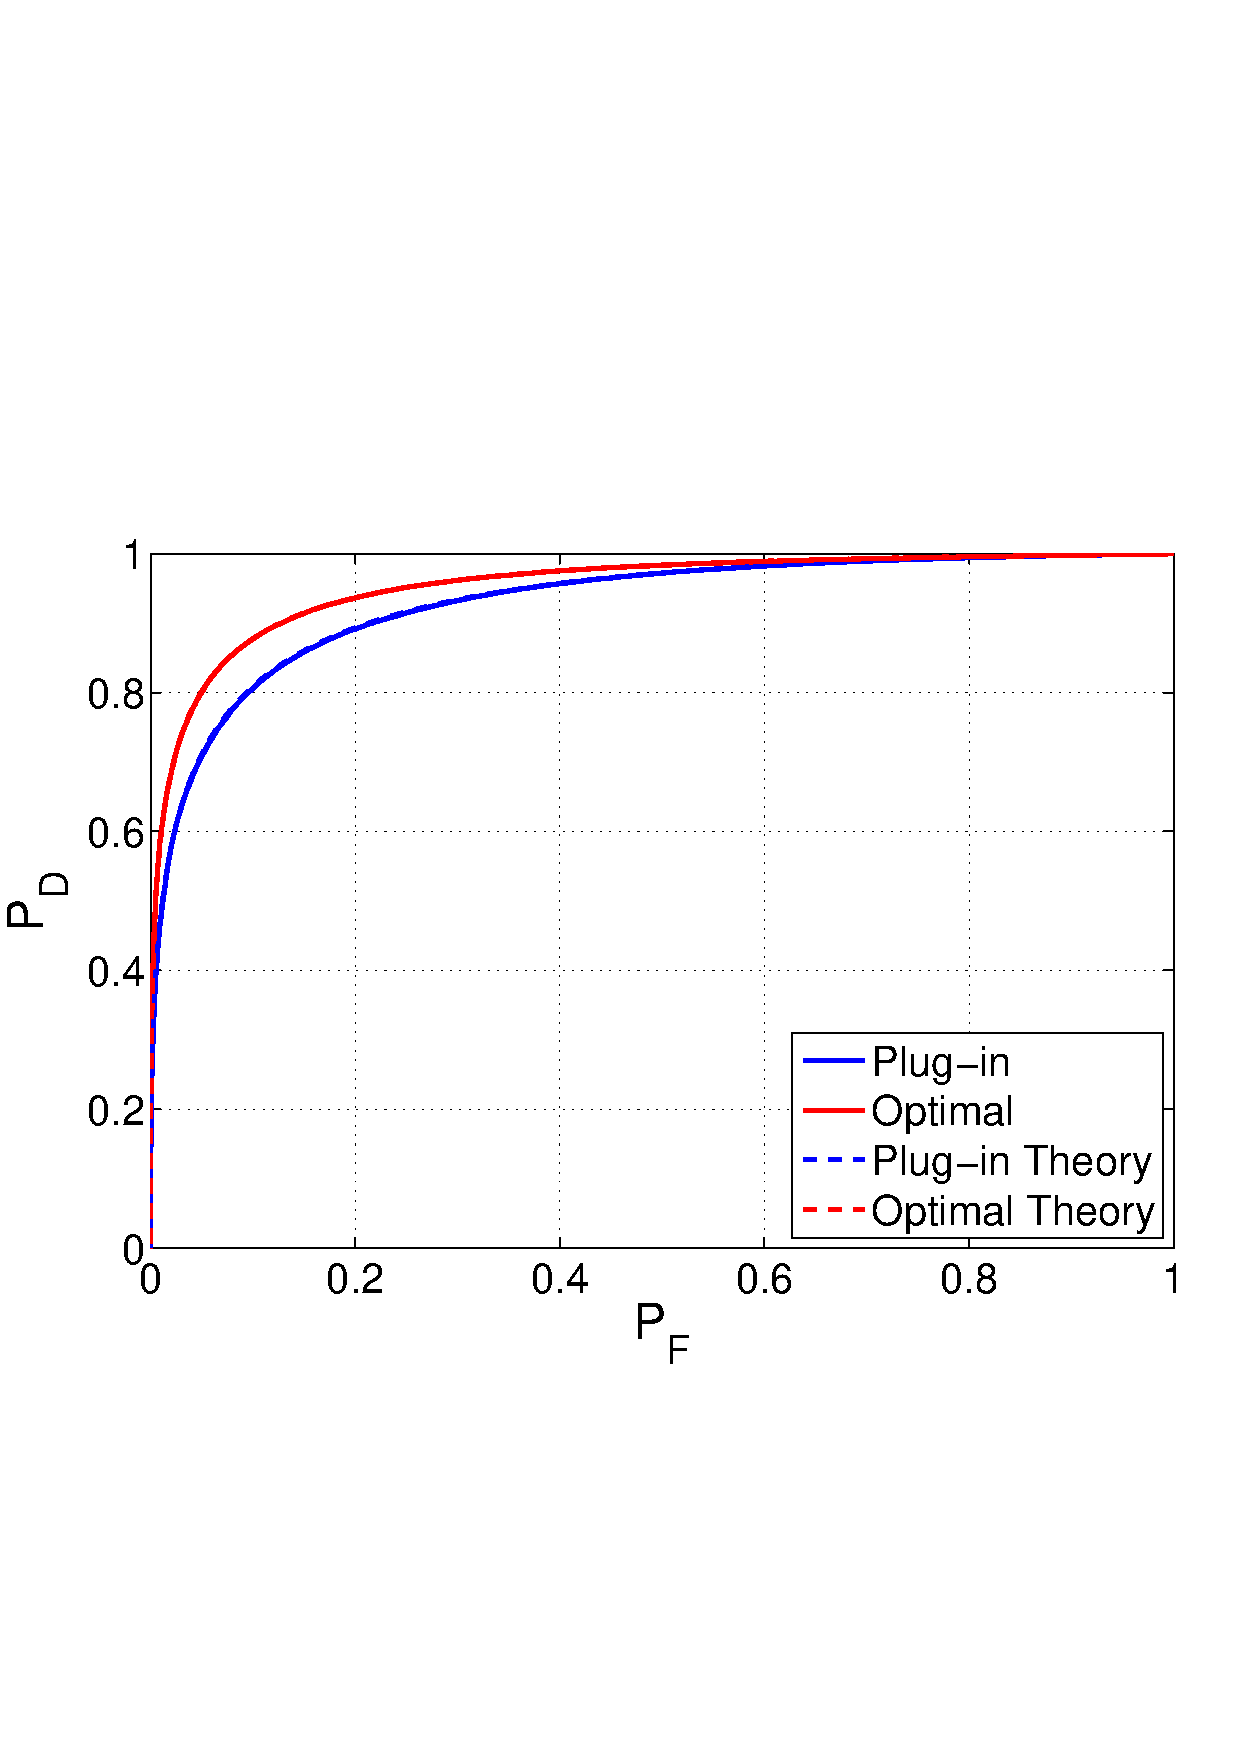
\includegraphics[width=3in]{figures/basic_roc.pdf}
\caption{Empirical and theoretical ROC curves for the plug-in and RMT matched subspace detectors. Empirical ROC curves were simulated with $n=500$, $m=500$, $k=2$, $\Sigma=\diag(3,0.1)$, and $p=0.8$. However, as $\sigma_2$ is below the critical threshold, $k_{\text{eff}} = 1$. The empirical ROC curves were computed using $5000$ test samples and averaged over 25 trials. $x$ was generated randomly for training samples but fixed for test samples. The theoretical ROC curves were obtained using (\ref{eq:roc}). Note the excellent agreement and the performance gain realized by the RMT detector.}\vskip-0.45cm
\label{fig:roc1}
\end{figure}


\subsection{ROC Curves}

We consider a setting where $k_{\text{eff}} = 1 < k = 2$. For this setting, as seen in Figure \ref{fig:roc1}, for any false alarm rate ($P_F$), the RMT detector achieves a higher probability of detection ($P_D$), demonstrating the sub-optimality of the plug-in detector. This is expected because $k_\text{eff}<k$ so that the plug-in detector is employing uninformative subspace components. The theoretical ROC curves in (\ref{eq:roc}) match the empirically generated ROC curves validating the performance predictions of (\ref{eq:roc}) which rely on Theorem \ref{th:angles}.

\subsection{Effect of Missing Data}
Figure \ref{fig:sparsity} examines the performance of each detector as a function of $p$. Again we observe the sub-optimality of the plug-in detector. The theoretical $P_D$ prediction in (\ref{eq:roc}) matches empirically achieved $P_D$ for both detectors. As expected, as $p$ decreases, the achieved probability of detection decreases. We note the presence of a critical $p_{\text{crit.}} : = \sqrt{c}/\max_{i}(\sigma_{i}^{2})$ obtained from Theorem \ref{th:angles}, below which (in the large system limit) we may only achieve $P_D=P_F$; the rounding in Figure \ref{fig:sparsity} is attributed to finite system approximation error.

\begin{figure}[t]
\centering
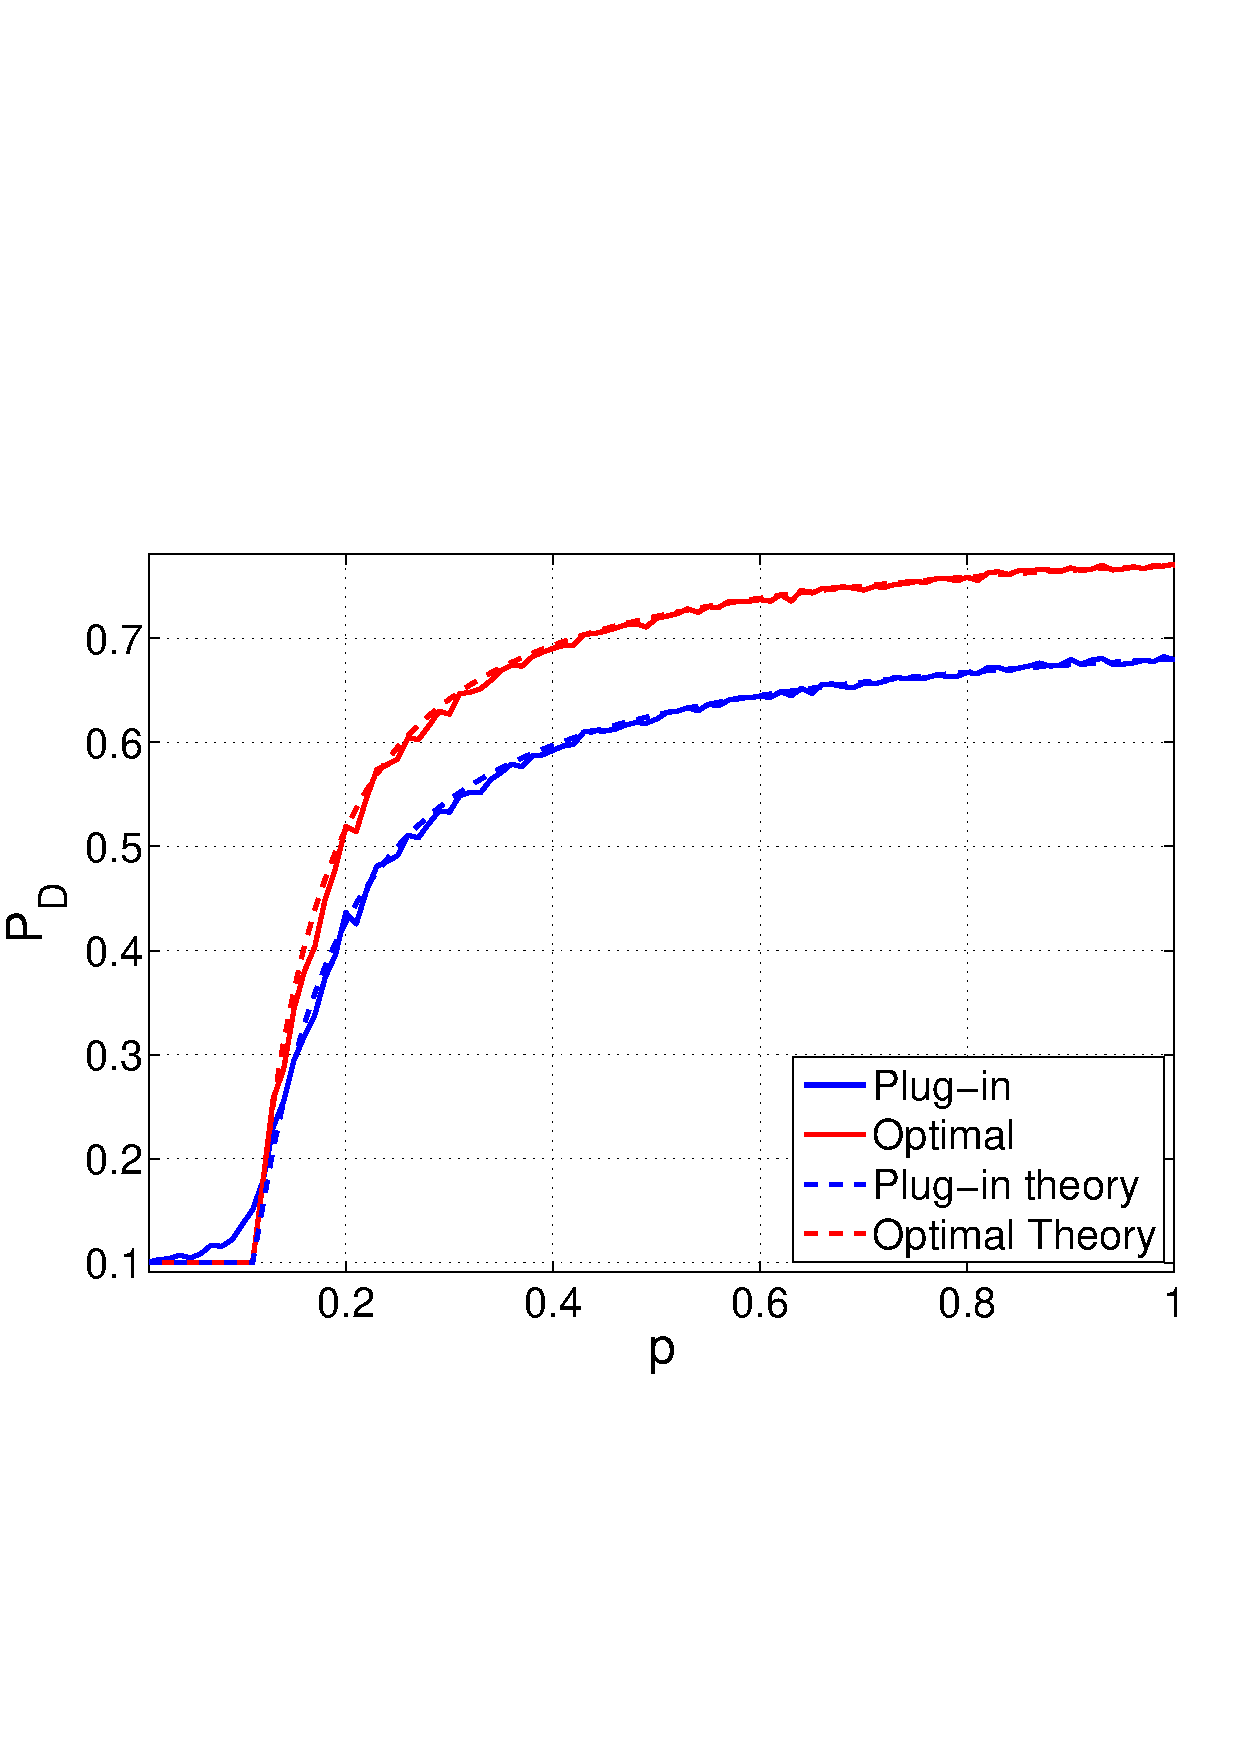
\includegraphics[width=3in]{figures/sparsity.pdf}
\caption{Empirically computed probability of detection, $P_D$, for a fixed probability of false alarm, $P_F=0.1$, for various $p$. Here, $n=1000$, $m=1000$, $k=2$, $\Sigma=\diag(3,0.1)$. $P_D$ was computed using (\ref{eq:roc}) and $x$ was generated as described in Figure \ref{fig:roc1}. For values of $p \leq 1/9$, $k_\text{eff}=0$ and performance degrades to $P_D = P_F +o(1)$ for both detectors. As $p$ increases, $k_\text{eff}=1$ allowing the detectors to achieve better than random guessing performance. When $k_\text{eff}>0$ the plug-in detector is sub-optimal for all values of $p$.}\vskip-0.45cm
\label{fig:sparsity}
\end{figure}

\section{Conclusion}\label{sec:conclusion}

We considered a deterministic MSD problem where the unknown low-rank signal subspace is estimated from noisy, limited, signal-bearing training data with missing entries.  We used RMT to characterize the resulting performance and showed that using $k_\text{eff} \leq k$ subspace components is optimal. The relationship between $k_{\text{eff}}$ and $p$ was made explicit in  Theorem \ref{th:angles} and we showed that detection better than random guessing (in the large system limit) is only achievable for $p > p_{\text{crit.}} : = \sqrt{c}/\max_{i}(\sigma_{i}^{2})$. 